% Tipo de documento y opciones.
\documentclass[11pt, a4paper]{article}


%---------------------------------------------------------------------------
%   PAQUETES
%---------------------------------------------------------------------------

% Idioma y codificación para Español.
\usepackage[utf8]{inputenc}
\usepackage[spanish, es-tabla, es-lcroman, es-noquoting]{babel}
\selectlanguage{spanish} 
%\usepackage[T1]{fontenc}

% Fuente utilizada.
\usepackage{courier}    % Fuente Courier.
\usepackage{microtype}  % Mejora la letra final de cara al lector.

% Diseño de página.
\usepackage{fancyhdr}   % Utilizado para hacer títulos propios.
\usepackage{lastpage}   % Referencia a la última página.
\usepackage{extramarks} % Marcas extras. Utilizado en pie de página y cabecera.
\usepackage[parfill]{parskip}    % Crea una nueva línea entre párrafos.
\usepackage{geometry}            % Geometría de las páginas.
\usepackage{cite}

% Símbolos y matemáticas.
\usepackage{amssymb, amsmath, amsthm, amsfonts, amscd}
\usepackage{upgreek}

% Otros.
\usepackage{enumitem}   % Listas mejoradas.
\usepackage[hidelinks]{hyperref}
\usepackage{graphicx}   % Gráficos.
\graphicspath{ {images/}}


%---------------------------------------------------------------------------
%   OPCIONES PERSONALIZADAS
%---------------------------------------------------------------------------

% Redefinir letra griega épsilon.
\let\epsilon\upvarepsilon

% Formato de texto.
\linespread{1.1}            % Espaciado entre líneas.
\setlength\parindent{0pt}   % No indentar el texto por defecto.
\setlist{leftmargin=.5in}   % Indentación para las listas.

% Estilo de página.
\pagestyle{fancy}
\fancyhf{}
\geometry{left=3cm,right=3cm,top=3cm,bottom=3cm,headheight=1cm,headsep=0.5cm}   % Márgenes y cabecera.


% Redefinir entorno de demostración (reducir espacio superior)
%\makeatletter
%\renewenvironment{proof}[1][\proofname] {\vspace{-15pt}\par\pushQED{\qed}\normalfont\topsep6\p@\@plus6\p@\relax\trivlist\item[\hskip\labelsep\it#1\@addpunct{.}]\ignorespaces}{\popQED\endtrivlist\@endpefalse}
%\makeatother

% Aumentar el tamaño del interlineado
\linespread{1.3}


%---------------------------------------------------------------------------
%   COMANDOS PERSONALIZADOS
%---------------------------------------------------------------------------

% Valor absoluto: \abs{}
\providecommand{\abs}[1]{\lvert#1\rvert}    

% Fracción grande: \ddfrac{}{}
\newcommand\ddfrac[2]{\frac{\displaystyle #1}{\displaystyle #2}}

% Texto en negrita en modo matemática: \bm{}
\newcommand{\bm}[1]{\boldsymbol{#1}}

% Línea horizontal.
\newcommand{\horrule}[1]{\rule{\linewidth}{#1}}

% Letras de conjuntos
\newcommand{\R}{\mathbb{R}}
\newcommand{\N}{\mathbb{N}}

% Sucesiones
\newcommand{\xn}{\{x_n\}}
\newcommand{\fn}{\{f_n\}}


%---------------------------------------------------------------------------
%   CABECERA Y PIE DE PÁGINA
%---------------------------------------------------------------------------

% Cabecera del documento.
\renewcommand\headrule{
	\begin{minipage}{1\textwidth}
		\hrule width \hsize 
	\end{minipage}
}

% Texto de la cabecera.
\lhead{\subject}  % Izquierda.
\chead{}            % Centro.
\rhead{\docauthor}    % Derecha.

% Pie de página del documento.
\renewcommand\footrule{                                 
	\begin{minipage}{1\textwidth}
		\hrule width \hsize   
	\end{minipage}\par
}

% Texto del pie de página.
\lfoot{}                                                 % Izquierda
\cfoot{}                                                 % Centro.
\rfoot{Página\ \thepage\ de\ \protect\pageref{LastPage}} % Derecha.


%---------------------------------------------------------------------------
%   ENTORNOS PARA MATEMÁTICAS
%---------------------------------------------------------------------------

% Nuevo estilo para definiciones.
\newtheoremstyle{definition-style} % Nombre del estilo.
{10pt}               % Espacio por encima.
{10pt}               % Espacio por debajo.
{}                   % Fuente del cuerpo.
{}                   % Identación.
{\bf}                % Fuente para la cabecera.
{.}                  % Puntuación tras la cabecera.
{.5em}               % Espacio tras la cabecera.
{\thmname{#1}\thmnumber{ #2}\thmnote{ (#3)}}     % Especificación de la cabecera (actual: nombre en negrita).

% Nuevo estilo para notas.
\newtheoremstyle{remark-style} 
{10pt}                
{10pt}                
{}                   
{}                   
{\itshape}          
{.}                  
{.5em}               
{}                  

% Nuevo estilo para teoremas y proposiciones.
\newtheoremstyle{theorem-style}
{10pt}                
{10pt}                
{\itshape}           
{}                  
{\bf}             
{.}                
{.5em}               
{\thmname{#1}\thmnumber{ #2}\thmnote{ (#3)}}                   

% Nuevo estilo para ejemplos.
\newtheoremstyle{example-style}
{10pt}                
{10pt}                
{}                  
{}                   
{\scshape}              
{:}                 
{.5em}               
{}                   

% Teoremas, proposiciones y corolarios.
\theoremstyle{theorem-style}
\newtheorem{nth}{Teorema}[section]
\newtheorem*{nprop}{Proposición}
\newtheorem{ncor}{Corolario}[section]

% Definiciones, ejercicios.
\theoremstyle{definition-style}
\newtheorem*{ndef}{Definición}
\newtheorem{ejer}{Ejercicio}

% Notas, soluciones.
\theoremstyle{remark-style}
\newtheorem*{nota}{Nota}
\newtheorem*{sol}{Solución}

% Ejemplos.
\theoremstyle{example-style}
\newtheorem{ejemplo}{Ejemplo}[section]

% Listas ordenadas con números romanos (i), (ii), etc.
\newenvironment{nlist}
{\begin{enumerate}
\renewcommand\labelenumi{(\emph{\roman{enumi})}}}
{\end{enumerate}}

% División por casos con llave a la derecha.
\newenvironment{rcases}
  {\left.\begin{aligned}}
  {\end{aligned}\right\rbrace}


%---------------------------------------------------------------------------
%   PÁGINA DE TÍTULO
%---------------------------------------------------------------------------

% Título del documento.
\newcommand{\subject}{}

% Autor del documento.
\newcommand{\docauthor}{}

% Título
\title{
  \normalfont \normalsize 
  \textsc{} \\ [25pt]    % Texto por encima.
  \horrule{0.5pt} \\[0.4cm] % Línea horizontal fina.
  \huge Algoritmos en exploración de grafos\\ \Large{Backtracking}\\ % Título.
  \horrule{2pt} \\[0.5cm] % Línea horizontal gruesa.
}

% Autor.
\author{\Large{Daniel Bolaños Martínez} 
\\\\
\Large{José María Borrás Serrano}
\\\\
\Large{Santiago de Diego de Diego}
\\\\
\Large{Fernando de la Hoz Moreno}}

% Fecha.
\date{\vspace{-1.5em} \normalsize }


%---------------------------------------------------------------------------
%   COMIENZO DEL DOCUMENTO
%---------------------------------------------------------------------------

\begin{document}

\maketitle  % Título.
\vfill
\begin{center}
\end{center}
\newpage
\newpage

\section{Análisis del problema}
El problema que tenemos ante nosotros es el problema de resolver un Sudoku. Un Sudoku consiste en un pasatiempo matemático que trata de rellenar con números del 1 al 9 una tabla de $9\times 9$ elementos, dividida en subcuadrículas de $3\times 3$, con casillas ya rellenadas previamente. Las normas que hay que cumplir son:
\begin{itemize}
\item No puede haber dos casillas en la misma fila con el mismo número
\item No puede haber dos casillas en la misma columna con el mismo número
\item No puede haber dos casillas, en la misma subcuadrícula de $3 \times 3$ con el mismo número.
\end{itemize}
Para resolver el problema tenemos que ir escribiendo números en las cuadrículas que se encuentran vacías sin romper las reglas anteriormente mencionadas. Se encontrará una solución cuando todas las casillas estén rellenas.

\section{Elección entre los métodos de Backtracking y Branch$\&$Bound}

La técnica que hemos escogido no puede ser Branch$\&$Bound debido a que no se puede realizar un cálculo de cotas, no podemos determinar que un nodo sea mejor que otro hasta que no lo hayamos recorrido.

Por eso hemos preferido escoger Bactracking, ya que la acción de visitar los nodos se hace de forma más eficaz.

\section{Diseño de la solución empleando la metodología Backtracking}

Para la resolución de dicho problema mediante la técnica de Backtracking. De forma general, los pasos para diseñar un algoritmo de Backtracking son:
\begin{itemize}
\item Buscar una representación del tipo $T=(x_1, x_2, \ldots, x_n)$ para las soluciones del problema.

En nuestro caso: $T(x_1, x_2, \dots, x_9)$ donde $x_i$ es la un vector de nueve componentes que representa la fila $i$ del sudoku.

\item Diseñar las restricciones implícitas, es decir, los valores que puede tener cada $x_i$ para contruir la solución.

En nuestro caso: $x_i$ $\in$ ${1, \dots, 9}$

\item Identificar las restricciones explícitas, es decir, las restricciones externas al proceso de encontrar la solución.

En nuestro ejemplo, no puede haber valores repetidos en una columna, en una fila o en un cuadrante.


\item Diseñar la estructura de árbol o grafo implícito que define los estados y transiciones entre estados de búsqueda de soluciones.

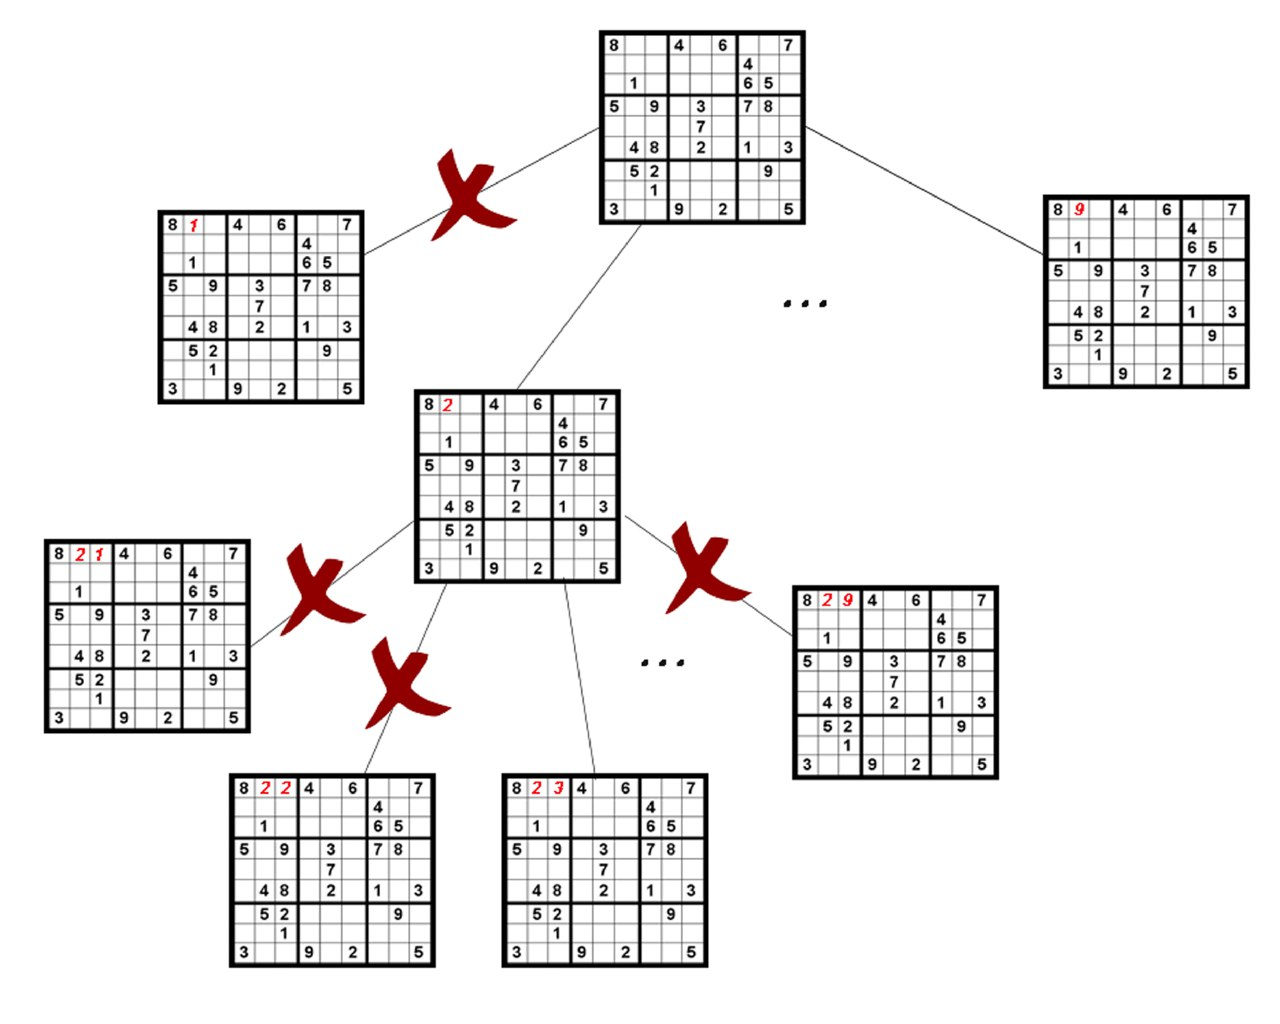
\includegraphics[scale=0.3]{Grafo_BackTracking}

\item Diseñar una función objetivo, la cual actuará como criterio de parada para encontrar las soluciones requeridas.

La función objetivo hace que el sudoku este completo, "sin huecos".


\item Diseñar una función de poda $B_k(x_1, x_2, \ldots, x_n)$ para eliminar la exploración de ramas que deriven en soluciones inadecuadas.

Si una de las ramas no cumple las restricciones explícitas, es decir, hay valores
repetidos en una columna, fila o cuadrante, se poda la rama.

\item Adaptar la estructura general del procedimiento Backtracking al problema y resolverlo.

\end{itemize}

\section{Pseudocódigo que soluciona el problema}

\begin{verbatim}
Funcion Backtracking(casilla c) devuelve booleano
    Si no quedan casillas libres entonces:
        Devolver Verdedero

    Para k de 1 al 9 hacer:
        Si esFactible(k):
            Poner k en casilla c
            Si no quedan casillas vacias:
                Devolver Verdadero
            Sino:
                Backtracking(SiguienteCasilla(c))

    Si ningunValorFactible :
        AnulaValor(c)
\end{verbatim}


\section{Explicación del funcionamiento del algoritmo sobre el ejemplo}

Vamos a tomar como ejemplo para explicar el funcionamiento del algoritmo un sudoku al cual sólo le faltan tres casillas:

\[
\begin{array}{ccccccccc}
0 & 0 & 4 & 6 & 7 & 8 & 9 & 1 & 2\\
6 & 7 & 2 & 0 & 9 & 5 & 3 & 4 & 8\\
1 & 9 & 8 & 3 & 4 & 2 & 5 & 6 & 7\\
8 & 5 & 9 & 7 & 6 & 1 & 4 & 2 & 3\\
4 & 2 & 6 & 8 & 5 & 3 & 7 & 9 & 1\\
7 & 1 & 3 & 9 & 2 & 4 & 8 & 5 & 6\\
9 & 6 & 1 & 5 & 3 & 7 & 2 & 8 & 4\\
2 & 8 & 7 & 4 & 1 & 9 & 6 & 3 & 5\\
3 & 4 & 5 & 2 & 8 & 6 & 1 & 7 & 9\\
\end{array}
\]

El algoritmo empieza seleccionando la primera casilla que tiene un 0, en este caso la casilla(0,0).
Una vez en la casilla comprueba si se puede poner un 1, no se puede ya que no cumple las restricciones. Comprueba si se puede poner un 2, tampoco es posible. Entonces comprueba si se puede poner un 3, esta vez sí cumple las restricciones por lo que en la casilla (0,0) pone un 3.

\[
\begin{array}{ccccccccc}
3 & 0 & 4 & 6 & 7 & 8 & 9 & 1 & 2\\
6 & 7 & 2 & 0 & 9 & 5 & 3 & 4 & 8\\
1 & 9 & 8 & 3 & 4 & 2 & 5 & 6 & 7\\
8 & 5 & 9 & 7 & 6 & 1 & 4 & 2 & 3\\
4 & 2 & 6 & 8 & 5 & 3 & 7 & 9 & 1\\
7 & 1 & 3 & 9 & 2 & 4 & 8 & 5 & 6\\
9 & 6 & 1 & 5 & 3 & 7 & 2 & 8 & 4\\
2 & 8 & 7 & 4 & 1 & 9 & 6 & 3 & 5\\
3 & 4 & 5 & 2 & 8 & 6 & 1 & 7 & 9\\
\end{array}
\]

Pasamos a la siguiente casilla vacía, la casilla (0,1). Vuelve a comprobar los números que se pueden colocar desde el 1 hasta el 9, ninguno de esos números verifica las restricciones. De esta forma en la casilla (0,1) no pone ningún número y la casilla se queda con un 0.

Como no hemos podido poner ningún número en la casilla volvemos a la casilla anterior, la (0,0), y se pone un 0.

\[
\begin{array}{ccccccccc}
0 & 0 & 4 & 6 & 7 & 8 & 9 & 1 & 2\\
6 & 7 & 2 & 0 & 9 & 5 & 3 & 4 & 8\\
1 & 9 & 8 & 3 & 4 & 2 & 5 & 6 & 7\\
8 & 5 & 9 & 7 & 6 & 1 & 4 & 2 & 3\\
4 & 2 & 6 & 8 & 5 & 3 & 7 & 9 & 1\\
7 & 1 & 3 & 9 & 2 & 4 & 8 & 5 & 6\\
9 & 6 & 1 & 5 & 3 & 7 & 2 & 8 & 4\\
2 & 8 & 7 & 4 & 1 & 9 & 6 & 3 & 5\\
3 & 4 & 5 & 2 & 8 & 6 & 1 & 7 & 9\\
\end{array}
\]

Seguimos probando con los números del 4 al 9, el 5 es un número válido así que lo pone en la casilla y pasa a la siguiente casilla vacía, la (0,1).

\[
\begin{array}{ccccccccc}
5 & 0 & 4 & 6 & 7 & 8 & 9 & 1 & 2\\
6 & 7 & 2 & 0 & 9 & 5 & 3 & 4 & 8\\
1 & 9 & 8 & 3 & 4 & 2 & 5 & 6 & 7\\
8 & 5 & 9 & 7 & 6 & 1 & 4 & 2 & 3\\
4 & 2 & 6 & 8 & 5 & 3 & 7 & 9 & 1\\
7 & 1 & 3 & 9 & 2 & 4 & 8 & 5 & 6\\
9 & 6 & 1 & 5 & 3 & 7 & 2 & 8 & 4\\
2 & 8 & 7 & 4 & 1 & 9 & 6 & 3 & 5\\
3 & 4 & 5 & 2 & 8 & 6 & 1 & 7 & 9\\
\end{array}
\]
 
En la casilla (0,1) volvemos a probar con los números del 1 al 9, el primer número válido es el 3 así que lo pone y pasa a la siguiente casilla vacía.

\[
\begin{array}{ccccccccc}
5 & 3 & 4 & 6 & 7 & 8 & 9 & 1 & 2\\
6 & 7 & 2 & 0 & 9 & 5 & 3 & 4 & 8\\
1 & 9 & 8 & 3 & 4 & 2 & 5 & 6 & 7\\
8 & 5 & 9 & 7 & 6 & 1 & 4 & 2 & 3\\
4 & 2 & 6 & 8 & 5 & 3 & 7 & 9 & 1\\
7 & 1 & 3 & 9 & 2 & 4 & 8 & 5 & 6\\
9 & 6 & 1 & 5 & 3 & 7 & 2 & 8 & 4\\
2 & 8 & 7 & 4 & 1 & 9 & 6 & 3 & 5\\
3 & 4 & 5 & 2 & 8 & 6 & 1 & 7 & 9\\
\end{array}
\]

Estamos en la casilla (0,3), comprobamos los números del 1 al 9 que son válidos, en este caso el número 1 cumple con todas las restricciones así que lo pone. Como no quedan casillas vacías el algoritmo termina.

\[
\begin{array}{ccccccccc}
5 & 3 & 4 & 6 & 7 & 8 & 9 & 1 & 2\\
6 & 7 & 2 & 1 & 9 & 5 & 3 & 4 & 8\\
1 & 9 & 8 & 3 & 4 & 2 & 5 & 6 & 7\\
8 & 5 & 9 & 7 & 6 & 1 & 4 & 2 & 3\\
4 & 2 & 6 & 8 & 5 & 3 & 7 & 9 & 1\\
7 & 1 & 3 & 9 & 2 & 4 & 8 & 5 & 6\\
9 & 6 & 1 & 5 & 3 & 7 & 2 & 8 & 4\\
2 & 8 & 7 & 4 & 1 & 9 & 6 & 3 & 5\\
3 & 4 & 5 & 2 & 8 & 6 & 1 & 7 & 9\\
\end{array}
\]


\section{Enunciado de un problema o caso real donde se pueda aplicar el algoritmo}

El algoritmo ha sido ideado inicialmente para resolver un sudoku, por tanto esta es su principal utilidad.  No obstante, es muy similar al algoritmo del coloreo de un grafo, el cual tiene numerosas aplicaciones prácticas. Ademas, algunos trabajos de investigación como \cite{sudoku}, presentan similitudes entre este problema y el \textit{Problema de Plegamiento de Proteínas} o el \textit{Problema del estado fundamental de los sistemas de hilado vítreo}.
\paragraph{}
El problema del sudoku puede resolverse también por el método del simplex, aunque nosotros nos hemos centrado solamente en emplear un algoritmo Backtracking.
\section{Cálculo del orden de eficiencia teórica del algoritmo }
La eficiencia del algoritmo en terminos recursivos es: $$ T(n) = 9*(9*3 + T(n-1))$$

Siendo n el número de casillas vacías que hay en el sudoku. Esto es porque en cada etapa recursiva, en el peor caso, se tendrá que calcular la factibilidad de los nueve valores posibles que puede tomar la casilla sobre la que se esta decidiendo. Para comprobar la factibilidad de cada valor se tiene que comparar con 9*3 casillas, viendo que no se repite dicho valor. Una vez hayado un valor factible para esa casilla se llama a resolver el sudoku con $n-1$ casillas vacías. Resolviendo la ecuación en recurrencias nos queda que: $$ T(n) = (1 - \frac{243}{1-9})*9^n + \frac{243}{1-9}$$ Que simplificando se nos queda: $$T(n) = 31.375*9^n - 30.375 $$



\section{Instrucciones sobre como compilar y ejecutar el código de la práctica}


\textbf{Compilación:} Ejecutar make en su terminal.

\textbf{Ejecución:} 

1. Crear un archivo de texto con el siguiente formato.
\begin{itemize}
\item Matriz con el sudoku a resolver (las casillas vacías se deben indicar como un 0).
\end{itemize}

Formato similar al proporcionado en dat/sudoku.dat

\[
\begin{array}{ccccccccc}
5 & 3 & 0 & 0 & 7 & 0 & 0 & 0 & 0\\
6 & 0 & 0 & 1 & 9 & 5 & 0 & 0 & 0\\
0 & 9 & 8 & 0 & 0 & 0 & 0 & 6 & 0\\
8 & 0 & 0 & 0 & 6 & 0 & 0 & 0 & 3\\
4 & 0 & 0 & 8 & 0 & 3 & 0 & 0 & 1\\
7 & 0 & 0 & 0 & 2 & 0 & 0 & 0 & 6\\
0 & 6 & 0 & 0 & 0 & 0 & 2 & 8 & 0\\
0 & 0 & 0 & 4 & 1 & 9 & 0 & 0 & 5\\
0 & 0 & 0 & 0 & 8 & 0 & 0 & 7 & 9\\
\end{array}
\]

Ejecutar el programa que se guardará por defecto en la carpeta bin del proyecto. 

./bin/prueba \textit{nombre\_archivo}
\begin{thebibliography}{X}
\bibitem{sudoku} \textsc{Mária Ercsey-Ravasz, Zoltán Toroczka}.
\textit{The Chaos Within Sudoku}.
Scientific Reports, Octubre 2012. Disponible en: \url{http://www.readcube.com/articles/10.1038/srep00725}
\end{thebibliography}	
\end{document}

\grid
\grid
\grid
\grid
